% !TeX encoding = UTF-8
% !TeX program = xelatex
\documentclass[12pt, a4paper]{article}
\usepackage{xeCJK} % 须放在\usepackage{}列中足够前的位置
\usepackage{fontspec}
\usepackage{graphicx}
\usepackage{caption}
\usepackage{enumerate}
\usepackage{setspace}
\usepackage{array} % 製作表格必須的宏包
\usepackage{tabularx} % 自動調整列寬的表格宏包
\usepackage{adjustbox}
\setCJKfamilyfont{heiti}{Heiti TC}
\CJKfamily{heiti}
\setmainfont{Arial}
\setstretch{1.5}


\begin{document}
\begin{center}
  {\Huge 邏輯設計實驗} \\[2.5cm]
  {\Huge Lab13} \\[1.5cm]
  {\Huge 同步計數器} \\ [4.5cm]
  \hspace{.6in}
  \begin{minipage}[t]{.4\linewidth}
    {\Large 班級:資訊一甲}\\[0.5cm]
    {\Large 學號:D1109023}\\[0.5cm]
    {\Large 姓名:楊孟憲}
  \end{minipage}    
\end{center}

\newpage

\begin{description}
  \fontsize{22pt}{25pt}\selectfont 
    \item [一、]摘要 
      \begin{enumerate}
        \fontsize{20pt}{22pt}\selectfont
          \item 同步計數器原理 \\
            \begin{samepage}
              \fontsize{16pt}{20}\selectfont
              \begin{description}
                \item [$\bullet$] 同步計數器中,所有的正反器由同一個時脈所觸發。
                \item [$\bullet$] 同步計數器時間延遲較短。
                \item [$\bullet$] 同步計數器可以用在較高之速度操作。
                \item [$\bullet$] 在計數狀態改變時,不會有暫態發生。 \\[.2cm]
                
\includegraphics[width=13cm]{./image/jk_flip_flop.png}
              \end{description}
            \end{samepage}

          \item 4-bit同步上/下數計數器設計-使用T 正反器 \\
            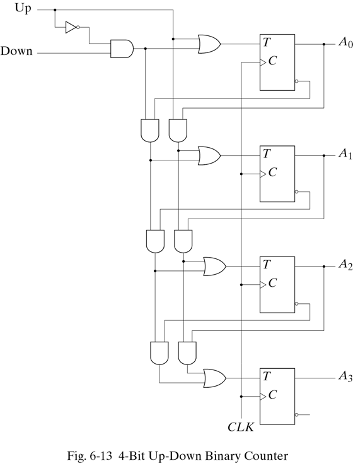
\includegraphics[width=13cm]{./image/t_flip_flop.png}
            
          \item 實驗 
            \begin{description}
              \fontsize{16pt}{20}\selectfont
                \item [(1)] 使用T正反器設計一個3-bit同步上/下數計數器
                \item [(2)] 設計一個 0~99 計數器 \\
              \normalsize  
            \end{description}
        \normalsize
      \end{enumerate}

    \item [二、]實驗結果
      \begin{description}
        \fontsize{20pt}{22pt}\selectfont
        \item 實驗一 (使用T正反器設計一個3-bit同步上/下數計數器)
            \begin{description}
              \fontsize{18pt}{20pt}
                \item [$\bullet$] Up/Down=0, 上數
                \item [$\bullet$] Up/Down=1, 下數
                \item []電路圖 \\[.3cm]
                  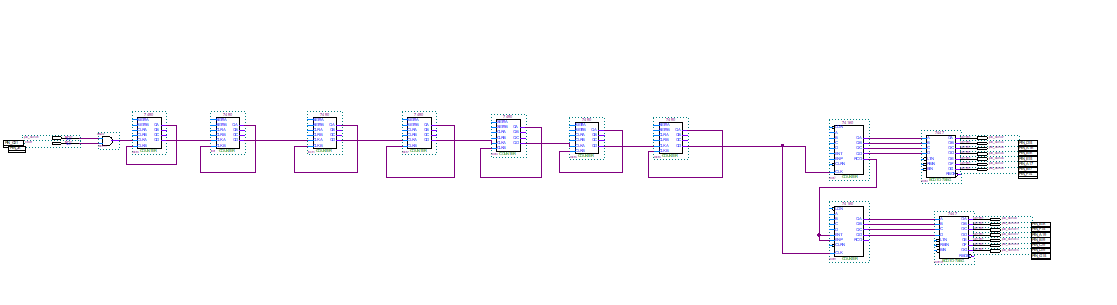
\includegraphics[width=13cm]{./image/ex1.png}
            \end{description}
          \normalsize
          
          \fontsize{20pt}{22pt}\selectfont
          \item 實驗二 (設計一個 0~99 計數器)
            \fontsize{16pt}{18pt}\selectfont
              \begin{description}
                \item [$\bullet$]請使用DE0所提供的 50MHz clock, CLOCK_50
                \item [$\bullet$] 將CLOCK_50 除頻 $10^7$,所得的 5Hz信號為此實驗的CLK\\
                \fontsize{18pt}{20pt}
                  \item []電路圖 \\[.3cm]
                    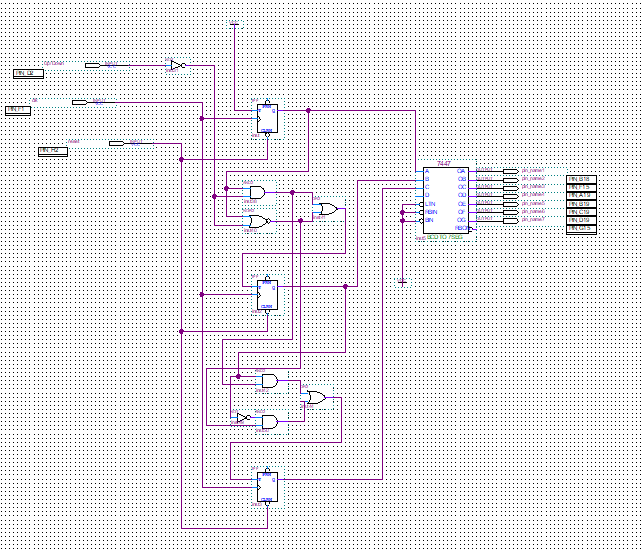
\includegraphics[width=13cm]{./image/ex2.png}
              \end{description}
            \normalsize
        \normalsize
      \end{description}
    \item [三、]問題討論心得 \\[.6cm]
      \begin{minipage}[t]{\linewidth}
        \fontsize{16}{18}\selectfont
        這次實驗我們使用T正反器成功地設計了一個3-bit同步上/下數計數器。透過適當的連接和時序控制。實驗二與上次實驗大致相同,要注意的是要將 start 判斷放在電路除頻率前
        。此次實驗讓我更深入理解了正反器的工作原理和數計數器的設計方法,並提升了我的數位電路設計能力。
      \end{minipage}
  \normalsize
\end{description}

\end{document}


